\documentclass[border=10pt]{standalone}

\usepackage{xcolor}

\definecolor{miamired}{RGB}{200,16,46}
\definecolor{darkgreen}{rgb}{0.09, 0.45, 0.27}
\definecolor{links}{HTML}{2A1B81}

\usepackage[export]{adjustbox}
\usepackage{amsfonts}
\usepackage{amsmath}
\usepackage{amssymb}
\usepackage{animate}
\usepackage{array}
\newcolumntype{M}[1]{>{\arraybackslash\hspace{0pt}}p{#1}}
\usepackage[justification=centering]{caption}
\usepackage{colortbl}
\usepackage{etoolbox}
\usepackage{fancybox}
\usepackage{forest}
\usepackage{fontawesome5}
\usepackage{framed}
\usepackage{graphics}
\usepackage{graphicx}
\graphicspath{ {Figures/} }
\usepackage{hyperref} 
\usepackage[utf8]{inputenc}
\usepackage{makecell}
\usepackage{mathtools}
\usepackage{marvosym}
\usepackage[framemethod=default]{mdframed}
%\addmediapath{ {Figures/} }
\usepackage{multicol}
%\usepackage{multimedia}
\usepackage{multirow}
\usepackage{pgfplots} %for tikzpictures
\pgfplotsset{compat=1.18}
\usepackage{sidecap}
\usepackage{smartdiagram}
\usepackage{soul}
\usepackage{subfigure}
\usepackage{tikz}
\usetikzlibrary{shapes.geometric, shapes, arrows}
\usepackage{times}
\urlstyle{same}
\usepackage{wasysym} % for smiley faces
\usepackage{wrapfig}


\usetikzlibrary{positioning}


\begin{document}


\begin{tikzpicture}[node distance = 2cm, auto]
	% Define block styles
	\tikzset{
		block/.style={rectangle, draw, fill=white, 
			text width=10em, text centered, rounded corners, minimum height=4em},
		line/.style={draw, -latex'}
	}
	% Place nodes
	\node [block] (a) {\textcolor{miamired}{\textbf{On-board Sensors}} \\ \faCar};
	\node [block, right=of a] (b) {\textcolor{miamired}{\textbf{Weather Conditions}} \\ \faCloud};
	\node [block, right=of b] (c) {\textcolor{miamired}{\textbf{Traffic and Road Conditions}} \\ \faRoad};
	\node [block, right=of c] (d) {\textcolor{miamired}{\textbf{Driver-specific Information}} \\ \faUser};
	
	\node [block, above=of b, above=of c] (transport) {\Large{\textbf{Transportation Data Sources}}};
	
	\node [block, below=of a] (a1) {\textbf{Example use cases:} \\ Track speed, \\ location, and \\ safety critical events};
	\node [block, below=of b] (b1) {\textbf{Example use cases:} \\ Extracted for a given route using \textbf{Weather APIs}};
	\node [block, below=of c] (c1) {\textbf{Example use cases:} \\ Used for routing \\ (i.e., A $\rightarrow$ B vs B $\rightarrow$ A)};
	\node [block, below=of d] (d1) {\textbf{Example use cases:} \\ Cameras, where eye gaze is used to detect driver fatigue};
	
	% Draw edges
	\path [line] (transport) -- (a);
	\path [line] (transport) -- (b);
	\path [line] (transport) -- (c);
	\path [line] (transport) -- (d);
	\path [line] (a) -- (a1);
	\path [line] (b) -- (b1);
	\path [line] (c) -- (c1);
	\path [line] (d) -- (d1);
\end{tikzpicture}


\end{document}